% Cara sistem bekerja untuk pelanggan dalam sehari: prediksi -> keputusan energi.
\documentclass[border=4pt]{standalone}
% Gaya bersama gambar deck Demo Day (dipakai semua gambar/*.tex standalone).
\usepackage{amssymb}
\usepackage{fontspec}
\setmainfont{DejaVu Sans Condensed}
\setsansfont{DejaVu Sans Condensed}
\newfontfamily\judulfont{DejaVu Sans}[BoldFont={DejaVu Sans Bold}, Ligatures=TeX]
\usepackage{tikz,pgfplots}
\pgfplotsset{compat=1.18, every axis/.append style={/pgf/number format/assume math mode=true, /pgf/number format/use comma, /pgf/number format/1000 sep={.}}}
\usetikzlibrary{positioning,arrows.meta,calc,shapes.geometric,fit,backgrounds}
\definecolor{gelap}{HTML}{15242B}
\definecolor{teal}{HTML}{285052}
\definecolor{amber}{HTML}{E8A317}
\definecolor{muda}{HTML}{DCE8E8}
\definecolor{abu}{HTML}{8A9499}
\definecolor{teks}{HTML}{1E2B30}
\definecolor{hijau}{HTML}{2F7D5B}
\definecolor{merah}{HTML}{A33A2A}
\color{teks}
\tikzset{
  ubin/.style={fill=muda, rounded corners=5pt, align=center, inner sep=6pt},
  inti/.style={ubin, fill=gelap, text=white},
  panah/.style={-{Stealth[length=3mm]}, line width=1.3pt, draw=amber},
  panahabu/.style={-{Stealth[length=2.5mm]}, line width=1pt, draw=abu},
  judulubin/.style={font=\judulfont\bfseries},
}
% Dibuat otomatis oleh buat_aset.py dari ml/results/energi_harian.json; jangan diedit manual.
\newcommand{\energiTurbin}{270}
\newcommand{\energiQa}{187}
\newcommand{\energiQb}{377}
\newcommand{\hariEnergi}{140}
\newcommand{\raspiWh}{71}
\newcommand{\chipWh}{4,1}
\newcommand{\raspiPersen}{26}
\newcommand{\chipPersen}{1,5}
\newcommand{\raspiPersenA}{19}
\newcommand{\raspiPersenB}{38}
\newcommand{\raspiPersenNum}{26.3}
\newcommand{\chipPersenNum}{1.5}
\newcommand{\hematKwh}{24}
\newcommand{\kaliHemat}{17}
\newcommand{\jRaspi}{182}
\newcommand{\jChip}{10,4}
\newcommand{\periodeEnergi}{2026-03-31--2026-10-20}

\AtBeginDocument{\hyphenpenalty=10000 \exhyphenpenalty=10000}

\begin{document}
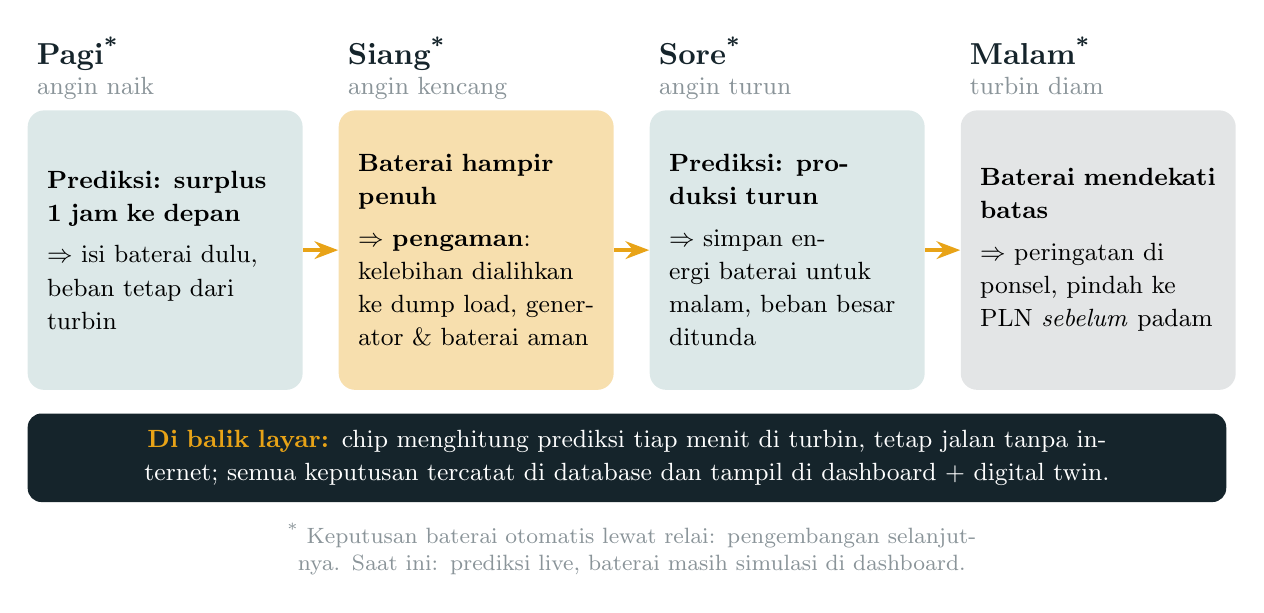
\begin{tikzpicture}[font=\fontsize{9.5}{12}\selectfont,
  langkah/.style={rounded corners=6pt, text width=3.0cm, minimum height=3.55cm, align=left, inner sep=7pt, anchor=north west},
  waktu/.style={font=\fontsize{9}{11}\selectfont, text=gelap, anchor=north west, align=left}]
  \def\kotak#1#2#3#4#5{%
    \node[waktu] at (#1,1.05) {#2};
    \node[langkah, fill=#3] (#5) at (#1,0) {#4};}
  \kotak{0}{{\judulfont\bfseries\fontsize{11}{13}\selectfont Pagi\textsuperscript{*}}\\{\color{abu}angin naik}}{muda}{\textbf{Prediksi: surplus 1 jam ke depan}\\[3pt]$\Rightarrow$ isi baterai dulu, beban tetap dari turbin}{s1}
  \kotak{3.95}{{\judulfont\bfseries\fontsize{11}{13}\selectfont Siang\textsuperscript{*}}\\{\color{abu}angin kencang}}{amber!35}{\textbf{Baterai hampir penuh}\\[3pt]$\Rightarrow$ \textbf{pengaman}: kelebihan dialihkan ke dump load, generator \& baterai aman}{s2}
  \kotak{7.9}{{\judulfont\bfseries\fontsize{11}{13}\selectfont Sore\textsuperscript{*}}\\{\color{abu}angin turun}}{muda}{\textbf{Prediksi: produksi turun}\\[3pt]$\Rightarrow$ simpan energi baterai untuk malam, beban besar ditunda}{s3}
  \kotak{11.85}{{\judulfont\bfseries\fontsize{11}{13}\selectfont Malam\textsuperscript{*}}\\{\color{abu}turbin diam}}{gelap!12}{\textbf{Baterai mendekati batas}\\[3pt]$\Rightarrow$ peringatan di ponsel, pindah ke PLN \emph{sebelum} padam}{s4}
  \foreach \a/\b in {s1/s2,s2/s3,s3/s4} \draw[panah] (\a.east) -- (\b.west);
  \node[inti, text width=14.8cm, anchor=north west, font=\fontsize{9.5}{12}\selectfont] at (0,-3.85)
    {\textcolor{amber}{\textbf{Di balik layar:}} chip menghitung prediksi tiap menit di turbin, tetap jalan tanpa internet; semua keputusan tercatat di database dan tampil di dashboard + digital twin.};
  \node[anchor=north, text=abu, text width=14.6cm, align=center, font=\fontsize{8.5}{10}\selectfont] at ([yshift=-4pt]current bounding box.south) {\textsuperscript{*} Keputusan baterai otomatis lewat relai: pengembangan selanjutnya. Saat ini: prediksi live, baterai masih simulasi di dashboard.};
\end{tikzpicture}
\end{document}
